\subsubsection{Drall} 
	\vspace{-1\baselineskip}
	\begin{flushright}	
		\begin{tabular}{|l|r|}
		\textbf{Type} 		 & Félin \\
		\textbf{Planete} 	 & Drall \\
		\textbf{Langage} 	 & Drallish \\
		\textbf{Orientation} & Neutre\\
		\end{tabular}
	\end{flushright}
	\vspace{-6\baselineskip}
	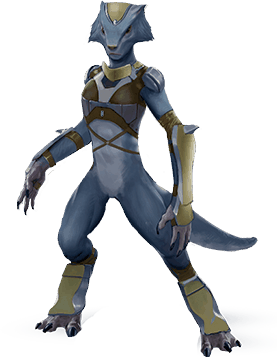
\includegraphics[width=6cm]{img/personnages/races/drall.png}

Les Dralls sont de petits mammifères (90~cm à 1,50~m), recouverts d’une fourrure brune et noire (gris pour les plus âgées), ils ont un museau et de grand yeux noirs. Les mains et les pieds se terminant par de petites griffes acérées. Les femelles sont généralement plus grandes et plus fortes. Les Drall ne portent pas de vêtements (comme toute créature à fourrure) et s’ornent de beaucoup de bijoux, ils cherchent constamment de nouvelles richesses quitte à se mettre hors la loi. Très avides de connaissances ils aiment apprendre juste pour le plaisir d’en savoir toujours plus.\\

\begin{description}[align=left]
\item[Soif de connaissance]    % +1
 	En tant qu’espèce, les Dralls sont surtout des êtres qui privilégient l’utilisation de leur cerveau à celle de leurs muscles. Ce sont des chercheurs à l’esprit méthodique, des observateurs studieux, et ils se considèrent eux-mêmes comme les meilleurs théoriciens de la galaxie. \\
 	\textit{d6 Intellect}

\item[Arsène Félin]    % +2
 	Le goût des Dralls pour les bijoux sans en avoir les moyens les ont poussés à devenir expert dans l’art de subtiliser tout ce qui brille. Ils ont donc un bonus naturel de +2 en Escalade, Crochetage et Discrétion \\
 	\textit{Atout Voleur}
 	
\item[Griffes rétractables]    % +1
	Leurs mains et leurs pieds sont terminés par de petites griffes très acérées.\\
	\textit{Arme naturelle (For+d6)}\\
    
\item[Vision Nocturne]  % +1
	Dans l’obscurité, les yeux des Dralls amplifient la lumière et ignorent les malus aux attaques pour des obscurités Légères ou Forte.\\
	\textit{Vision nocturne}\\

\item[Mourir moins bête]       % -2
 	Le personnage veut tout savoir. Dès qu’un Drall découvre quelque chose de nouveau, il ne peut pas s’empêcher de s’y intéresser.\\
    \textit{Handicap Curieux} \\

\item[Frêle]       				% -2
 	Les Dralls sont des intellectuels, agiles de par leur nature, mais ils ne sont pas taillés pour le combat. Ils ont tendance à faire usage de la ruse pour esquiver les affrontements physiques.\\
    \textit{Handicap Frêle (-1 Résistance)}
\end{description}

